\Exhibit{MediumDistributedExplained}{%
    Скриншоты популярных блогов, объясняющих, что метка `Distributed'
    это знак отбора статьи редакторами Medium%
}

Справочный центр Medium не объяснял, как распознать, что статья отобрана редакторами.
Вместо этого можно использовать статьи в популярных блогах.
Приводим несколько источников для надёжности.

`Better Marketing' это издание на Medium со 119 тысячами подписчиков:

\begin{center}
    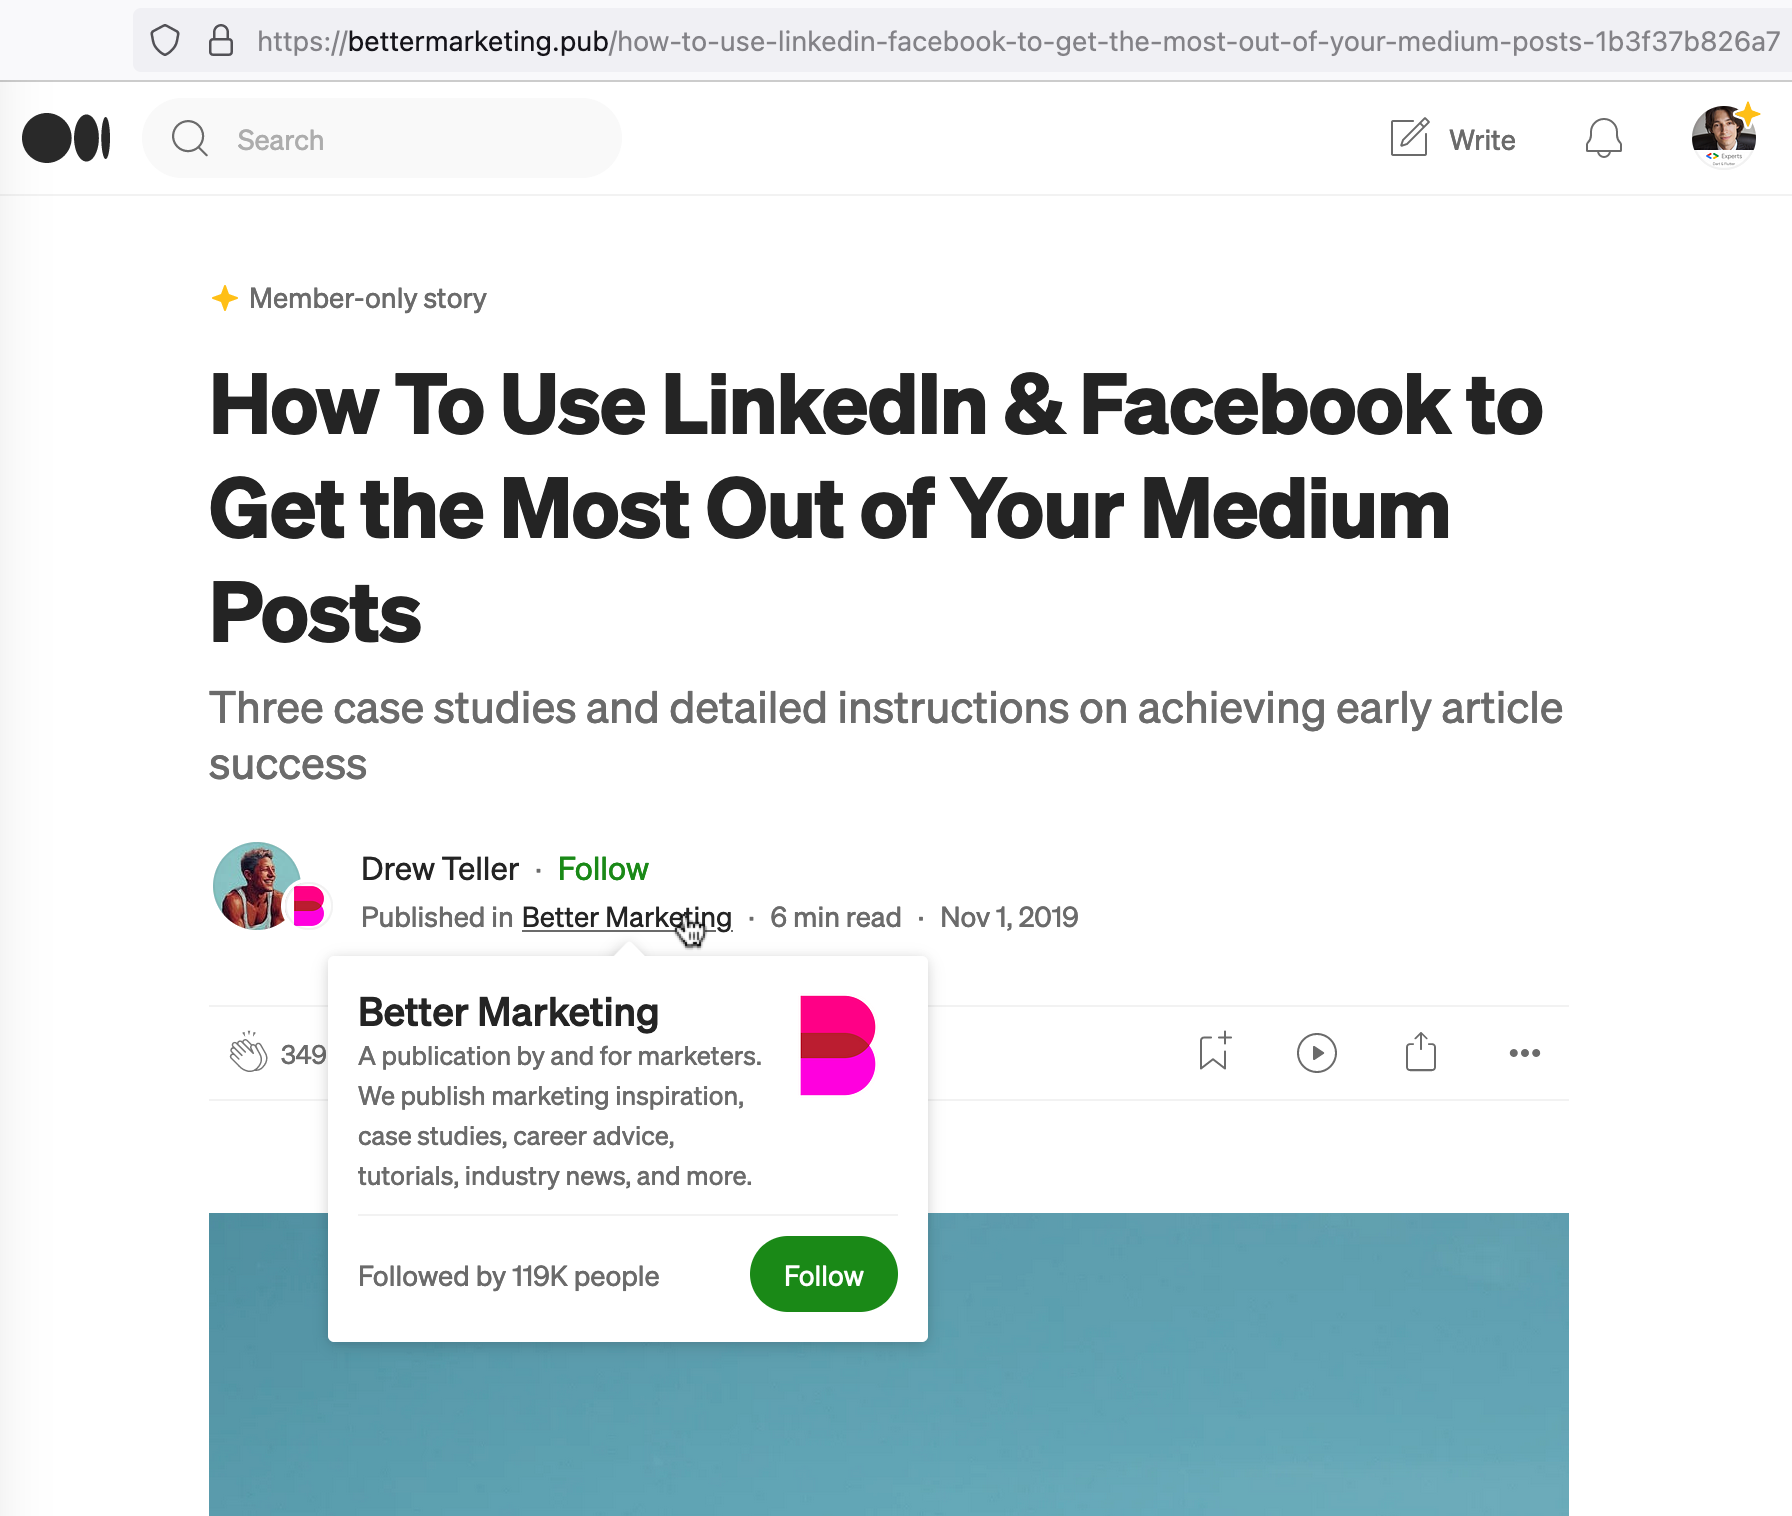
\includegraphics[width=\textwidth]{bettermarketing-top}
\end{center}

Оно опубликовало статью, где в середине объясняется это:

\begin{center}
    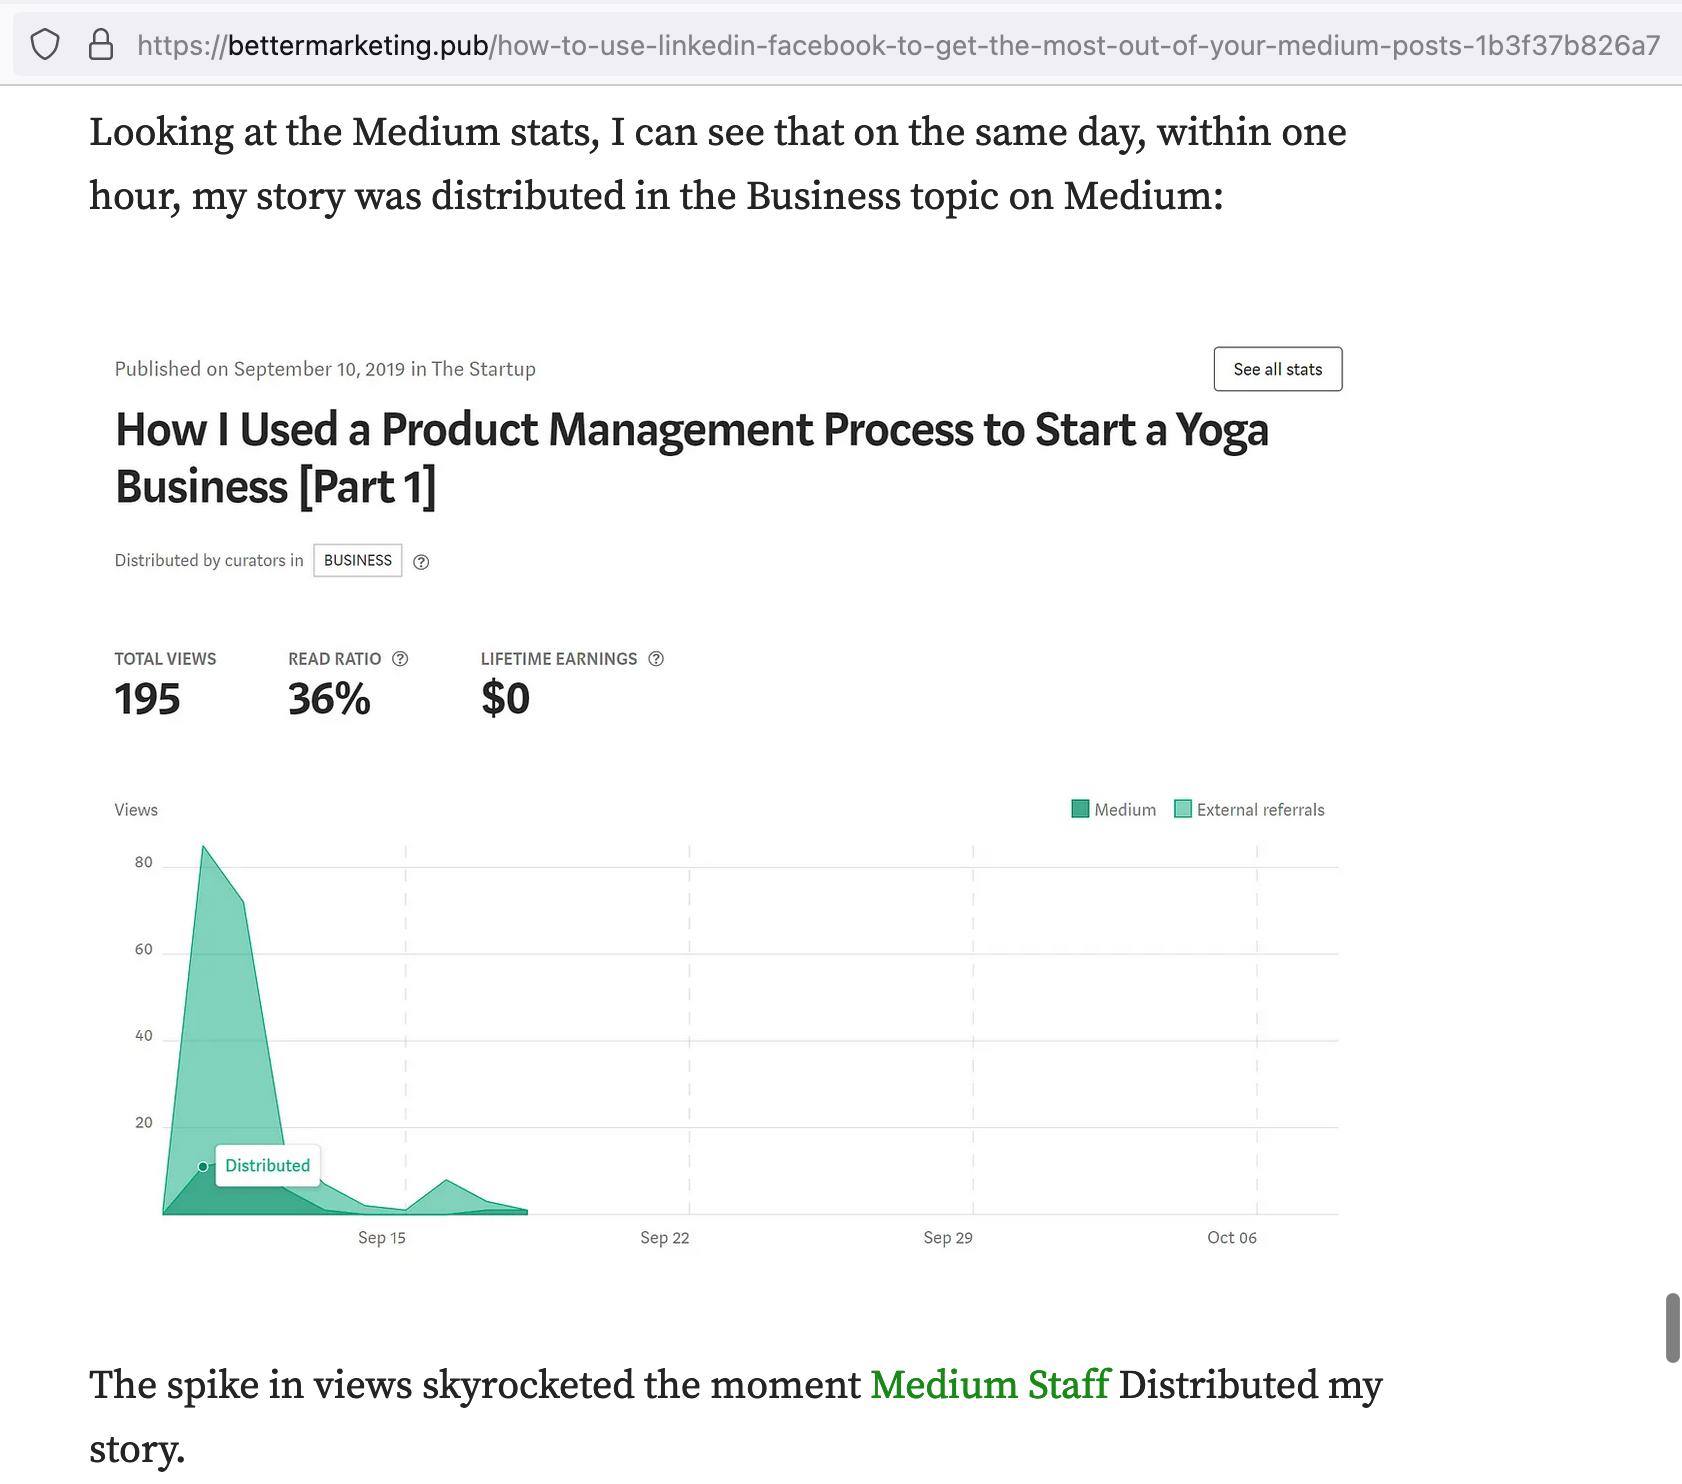
\includegraphics[width=\textwidth]{bettermarketing-content}
\end{center}
\pagebreak


Пост на TheSideBlogger.com подтверждает это и напрямую подсвечивает знак.
Он также подтверждает, что программа прекратилась в середине 2022.

\begin{center}
    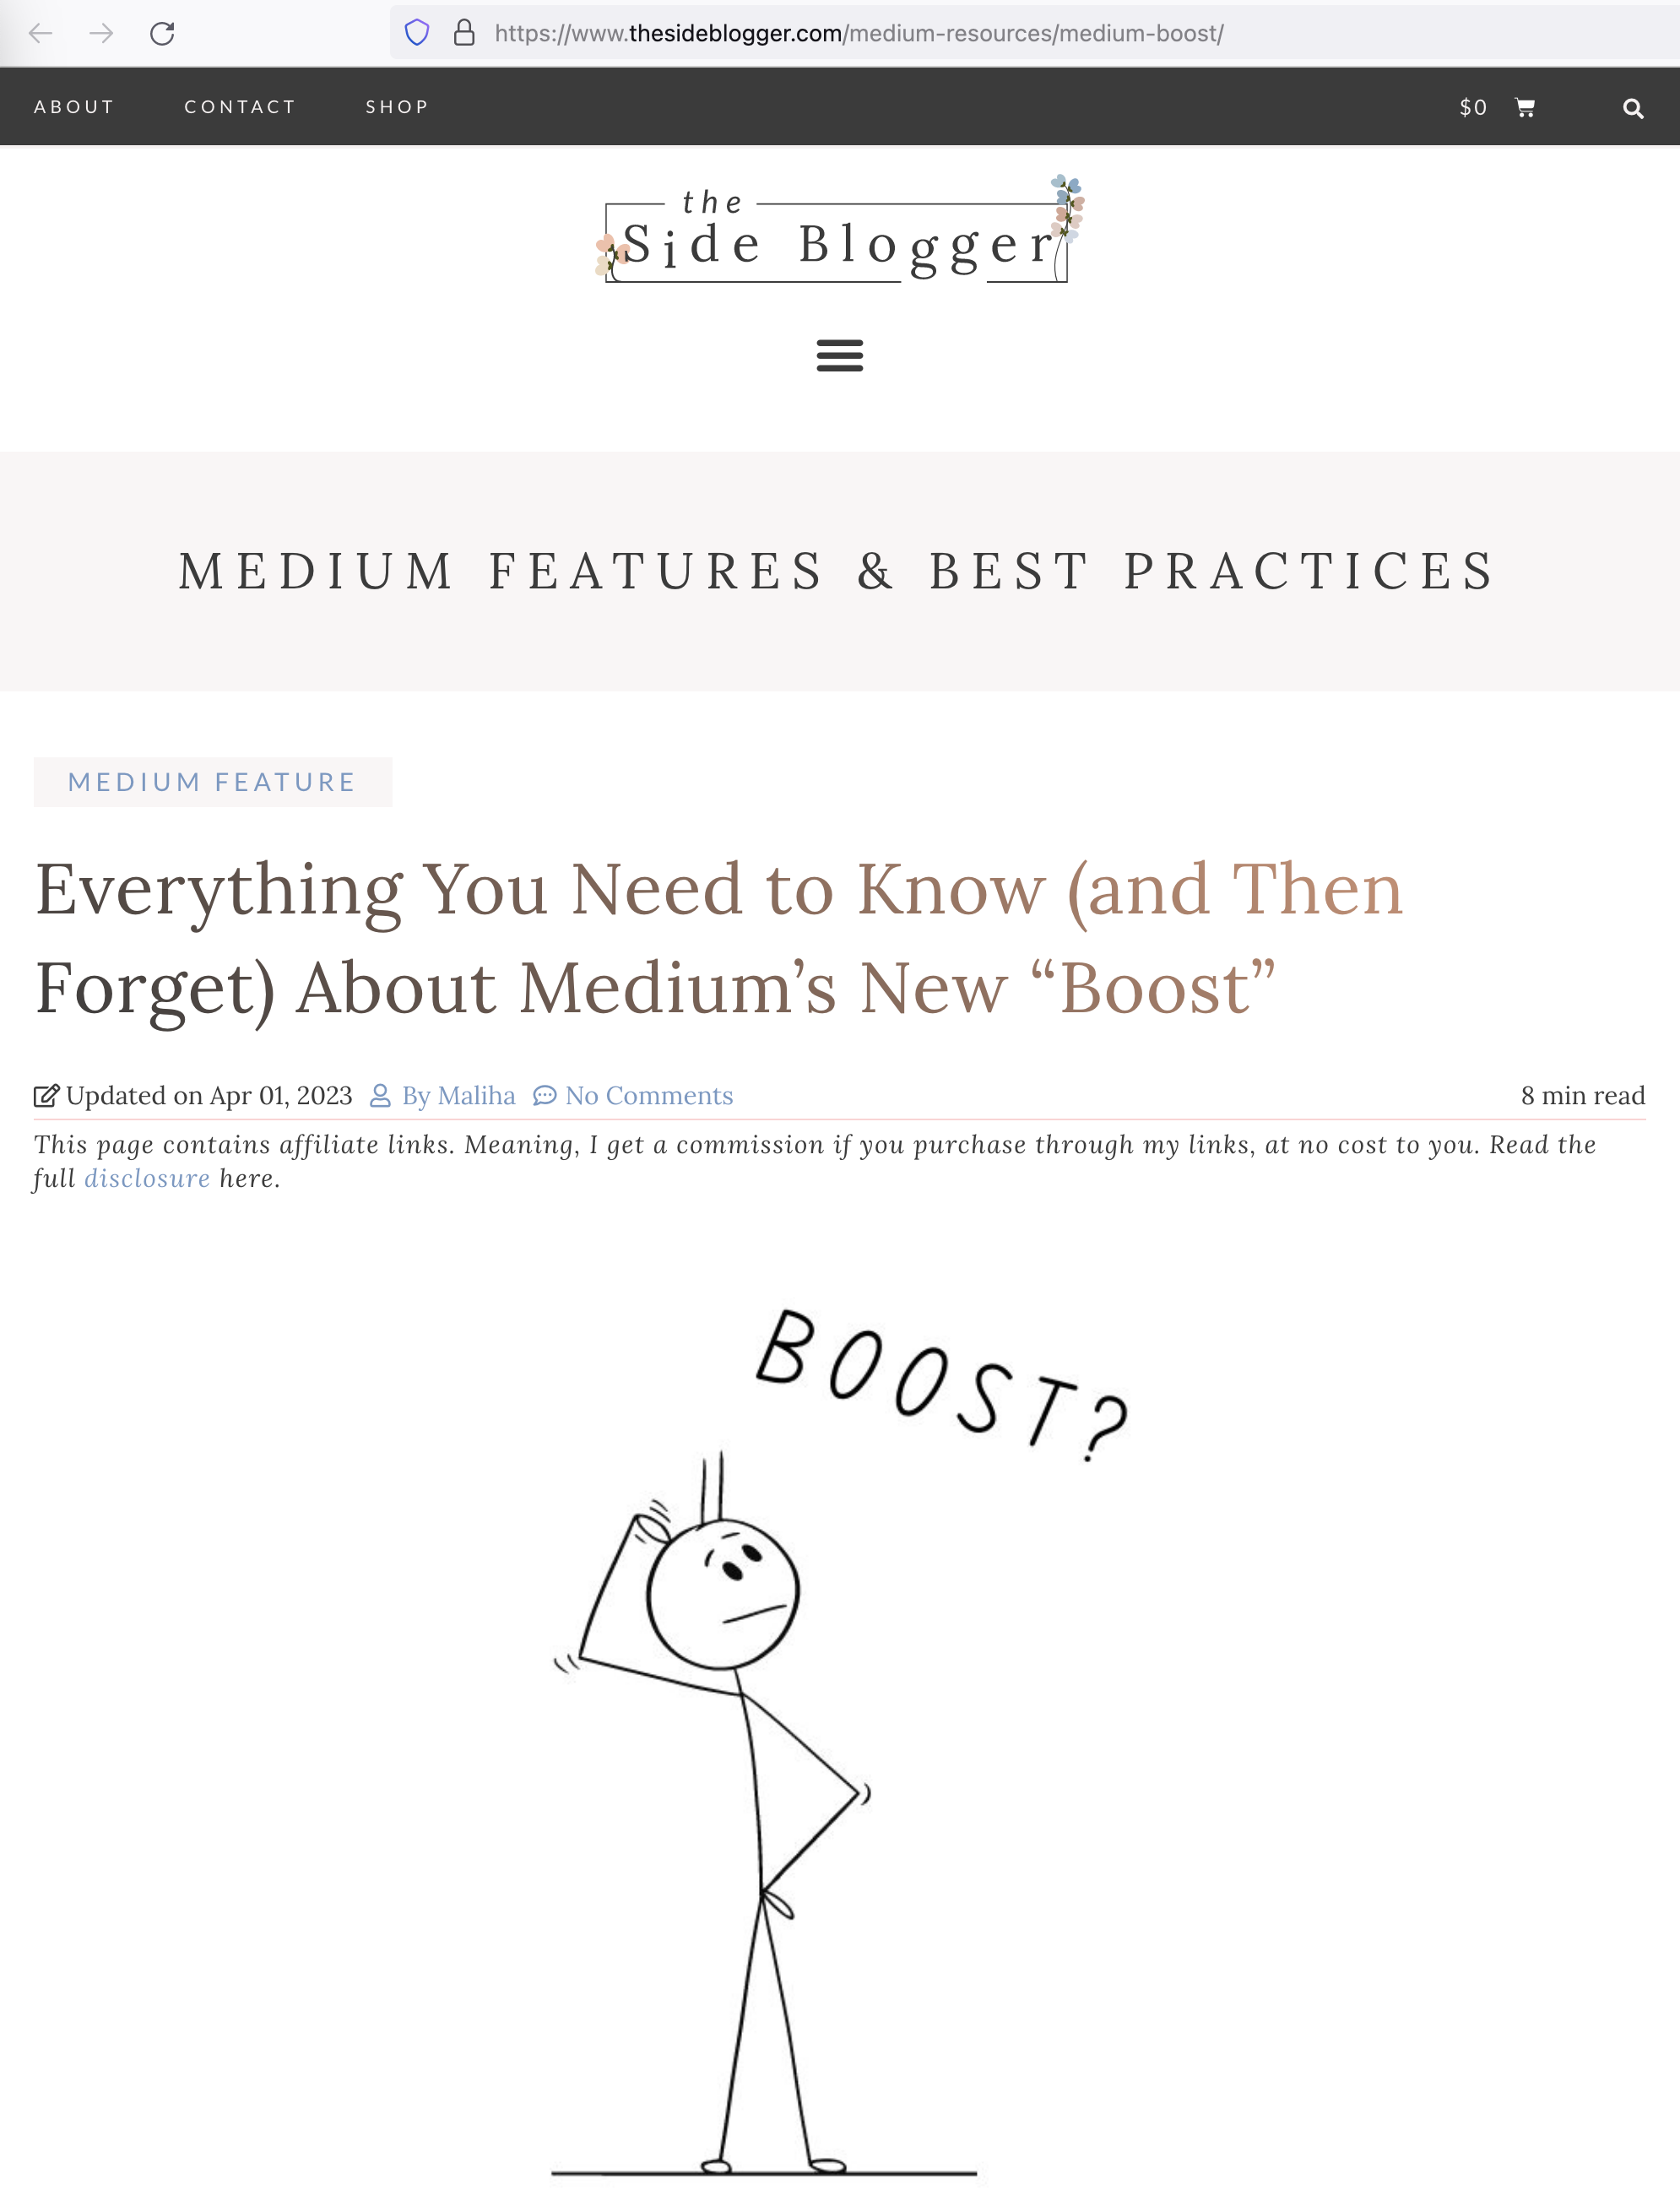
\includegraphics[width=38em]{thesideblogger-p1}
\end{center}
\WillContinue
\pagebreak

\Continuing
\begin{center}
    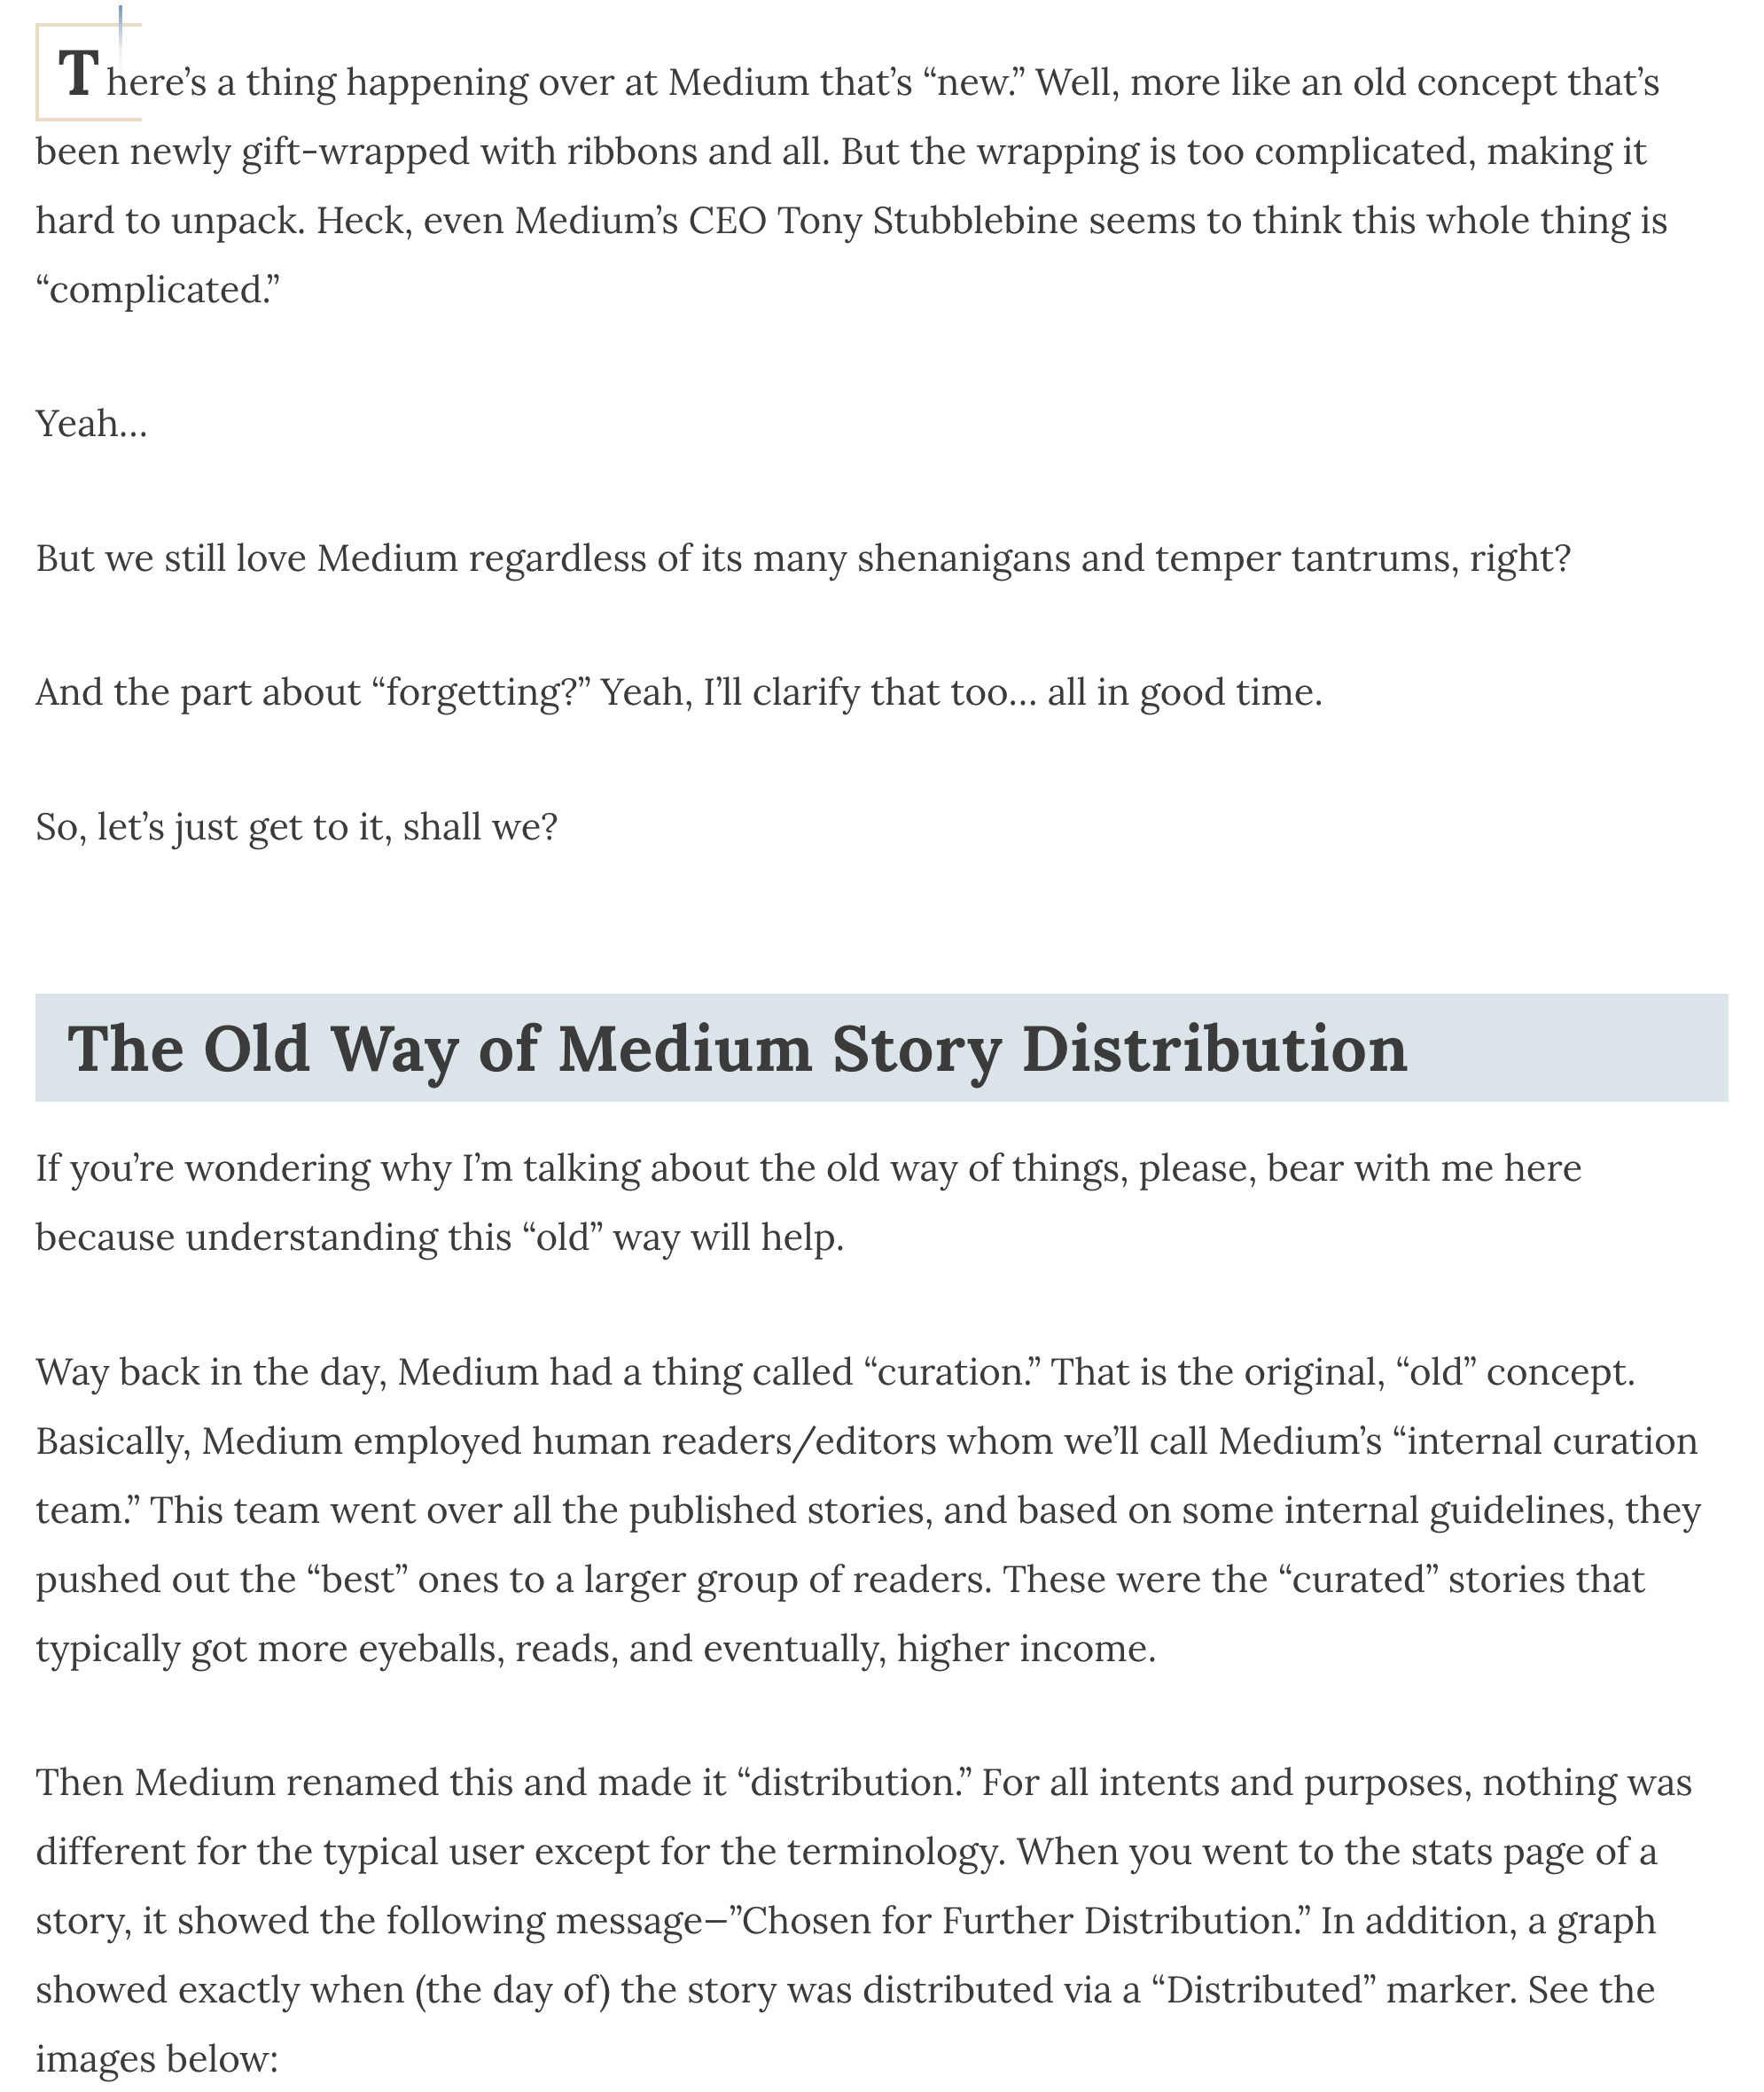
\includegraphics[width=\textwidth]{thesideblogger-p2}
\end{center}
\WillContinue
\pagebreak

\Continuing
\begin{center}
    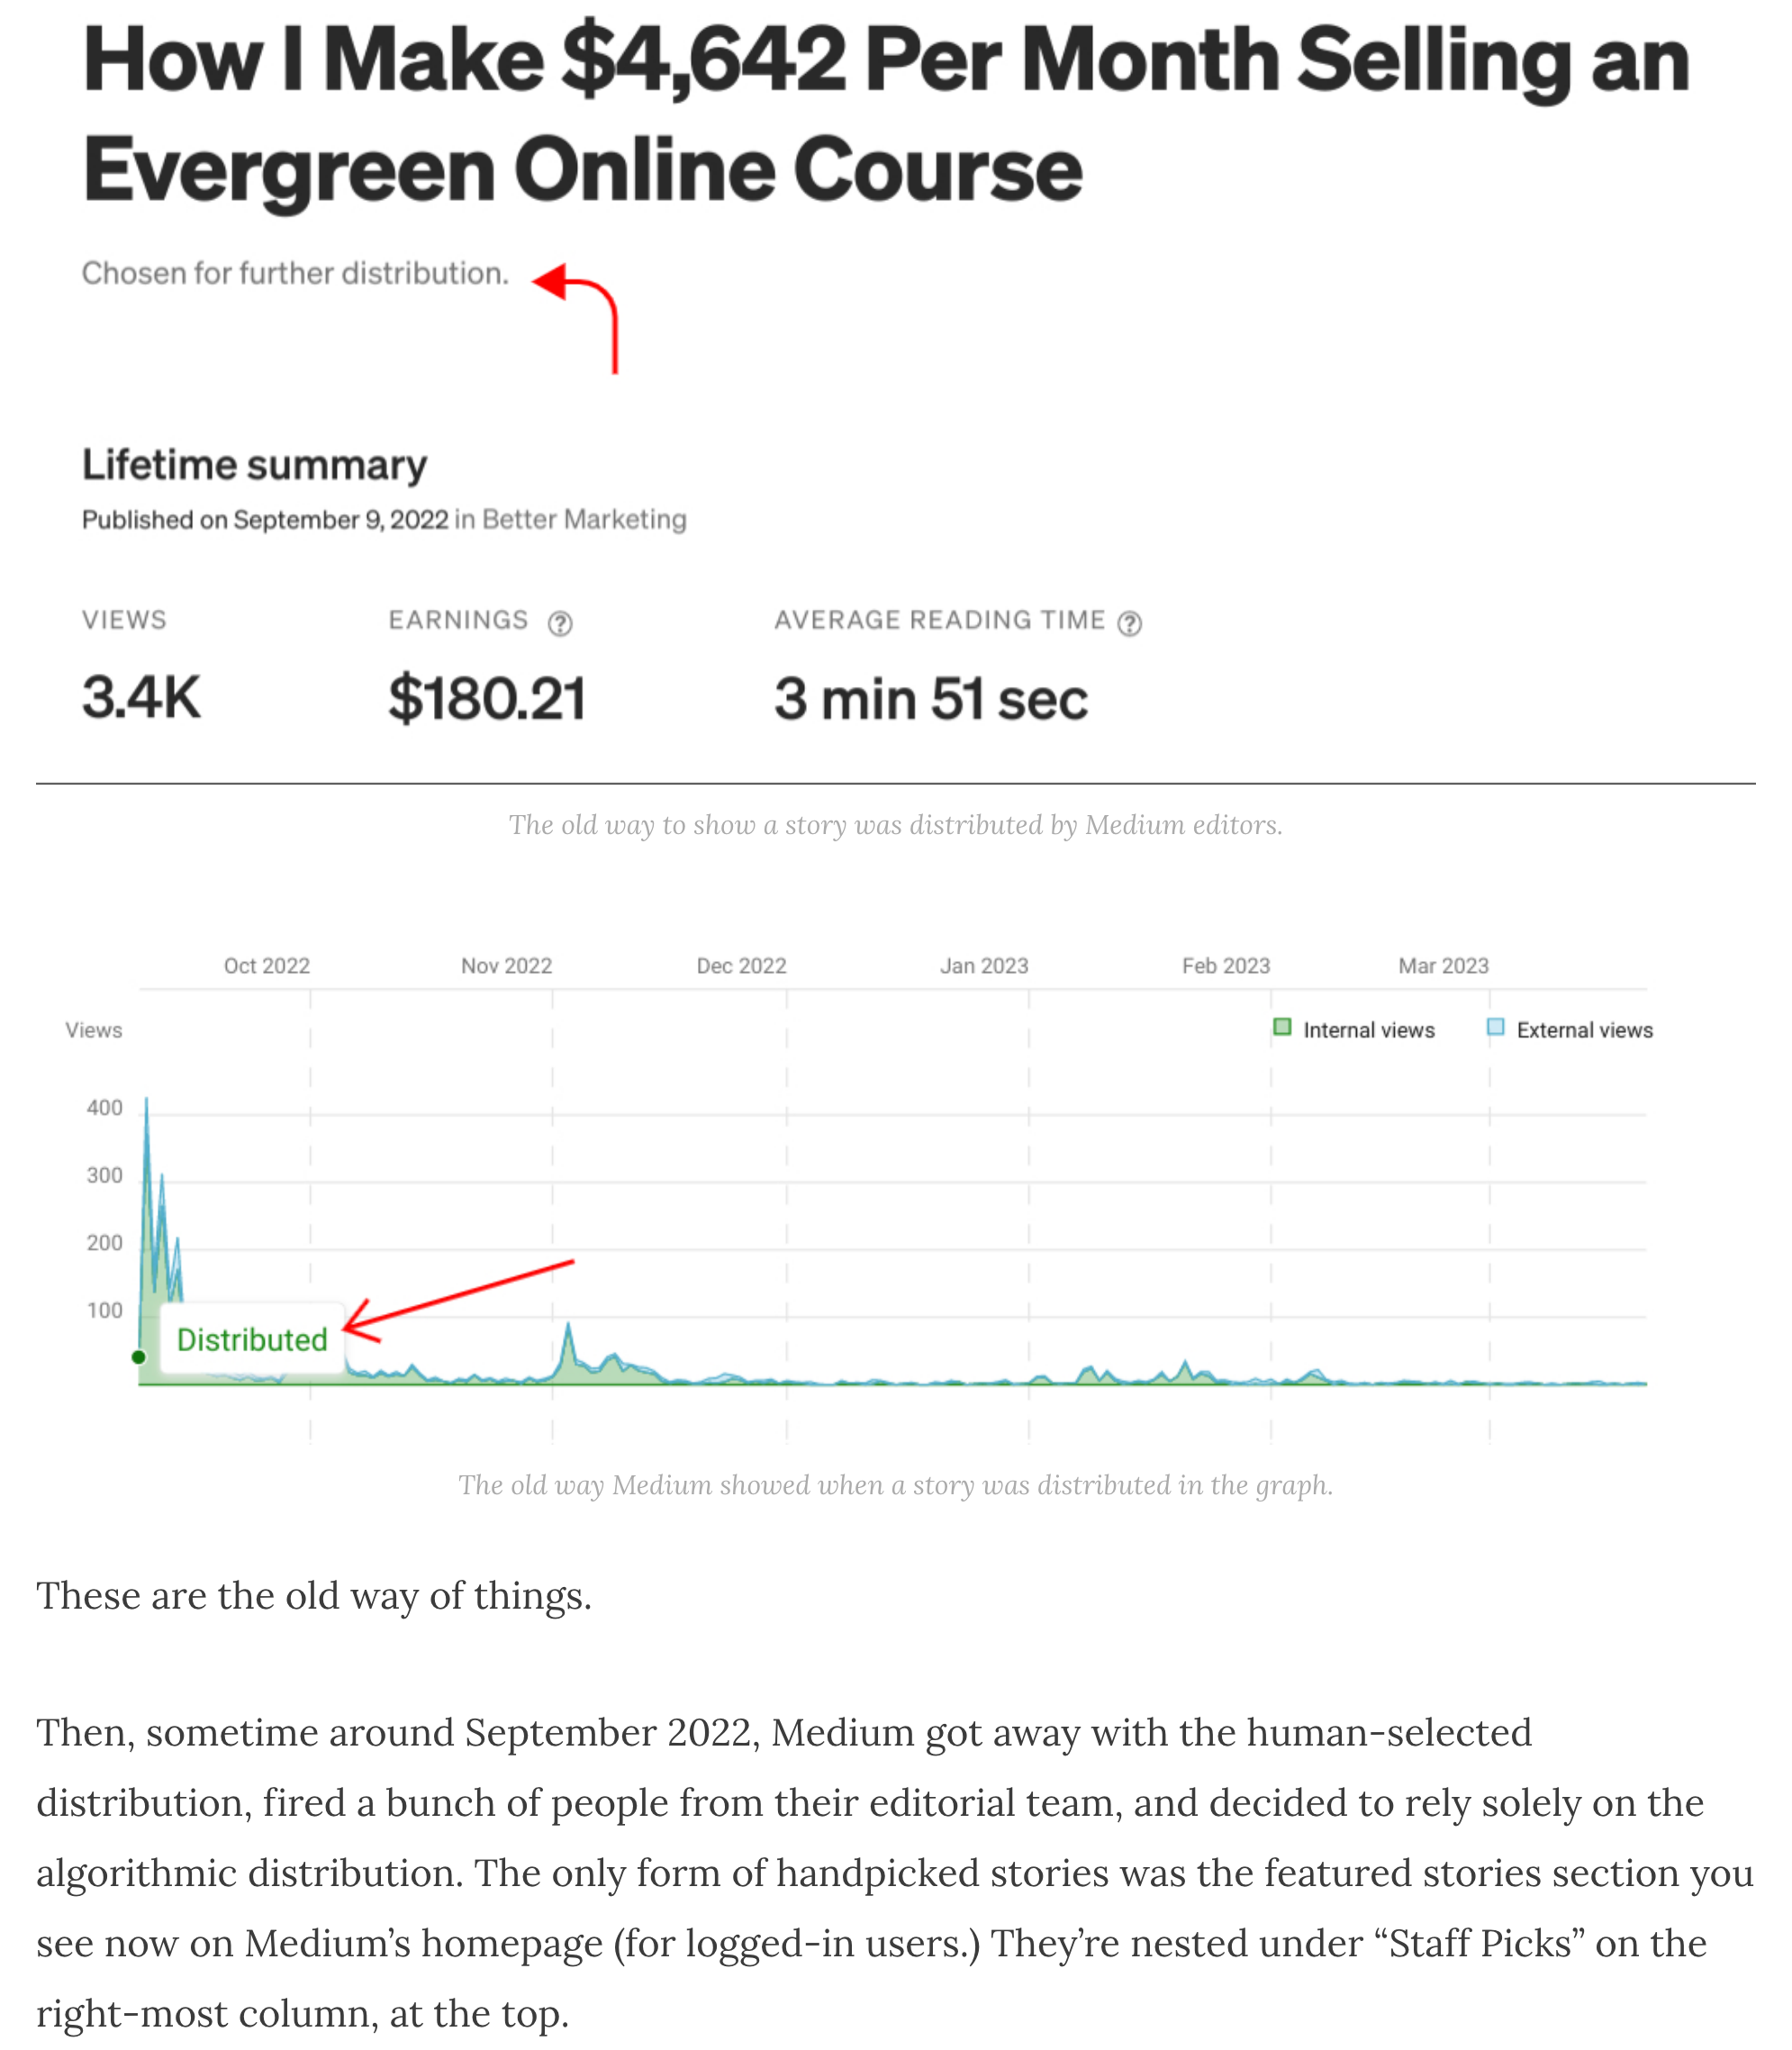
\includegraphics[width=\textwidth]{thesideblogger-p3}
\end{center}
\pagebreak


В сентябре 2022 в одном из официальных блогов на Medium
было объявлено, что они убирают один из двух признаков:

\ParagraphQuote{%
    \dots Это также означает, что для более широкого показа статьи теперь не отбираются вручную\dots

    Мы решили перестать показывать надпись `отобрано для широкого распространения'
    на странице статистики.%
}

Это потому, что они запустили алгоритм, чтобы упростить работу редакторов.
Это оставляет метку \Quote{Distributed} на графике единственным признаком ручного отбора статьи в старой программе.

\begin{center}
    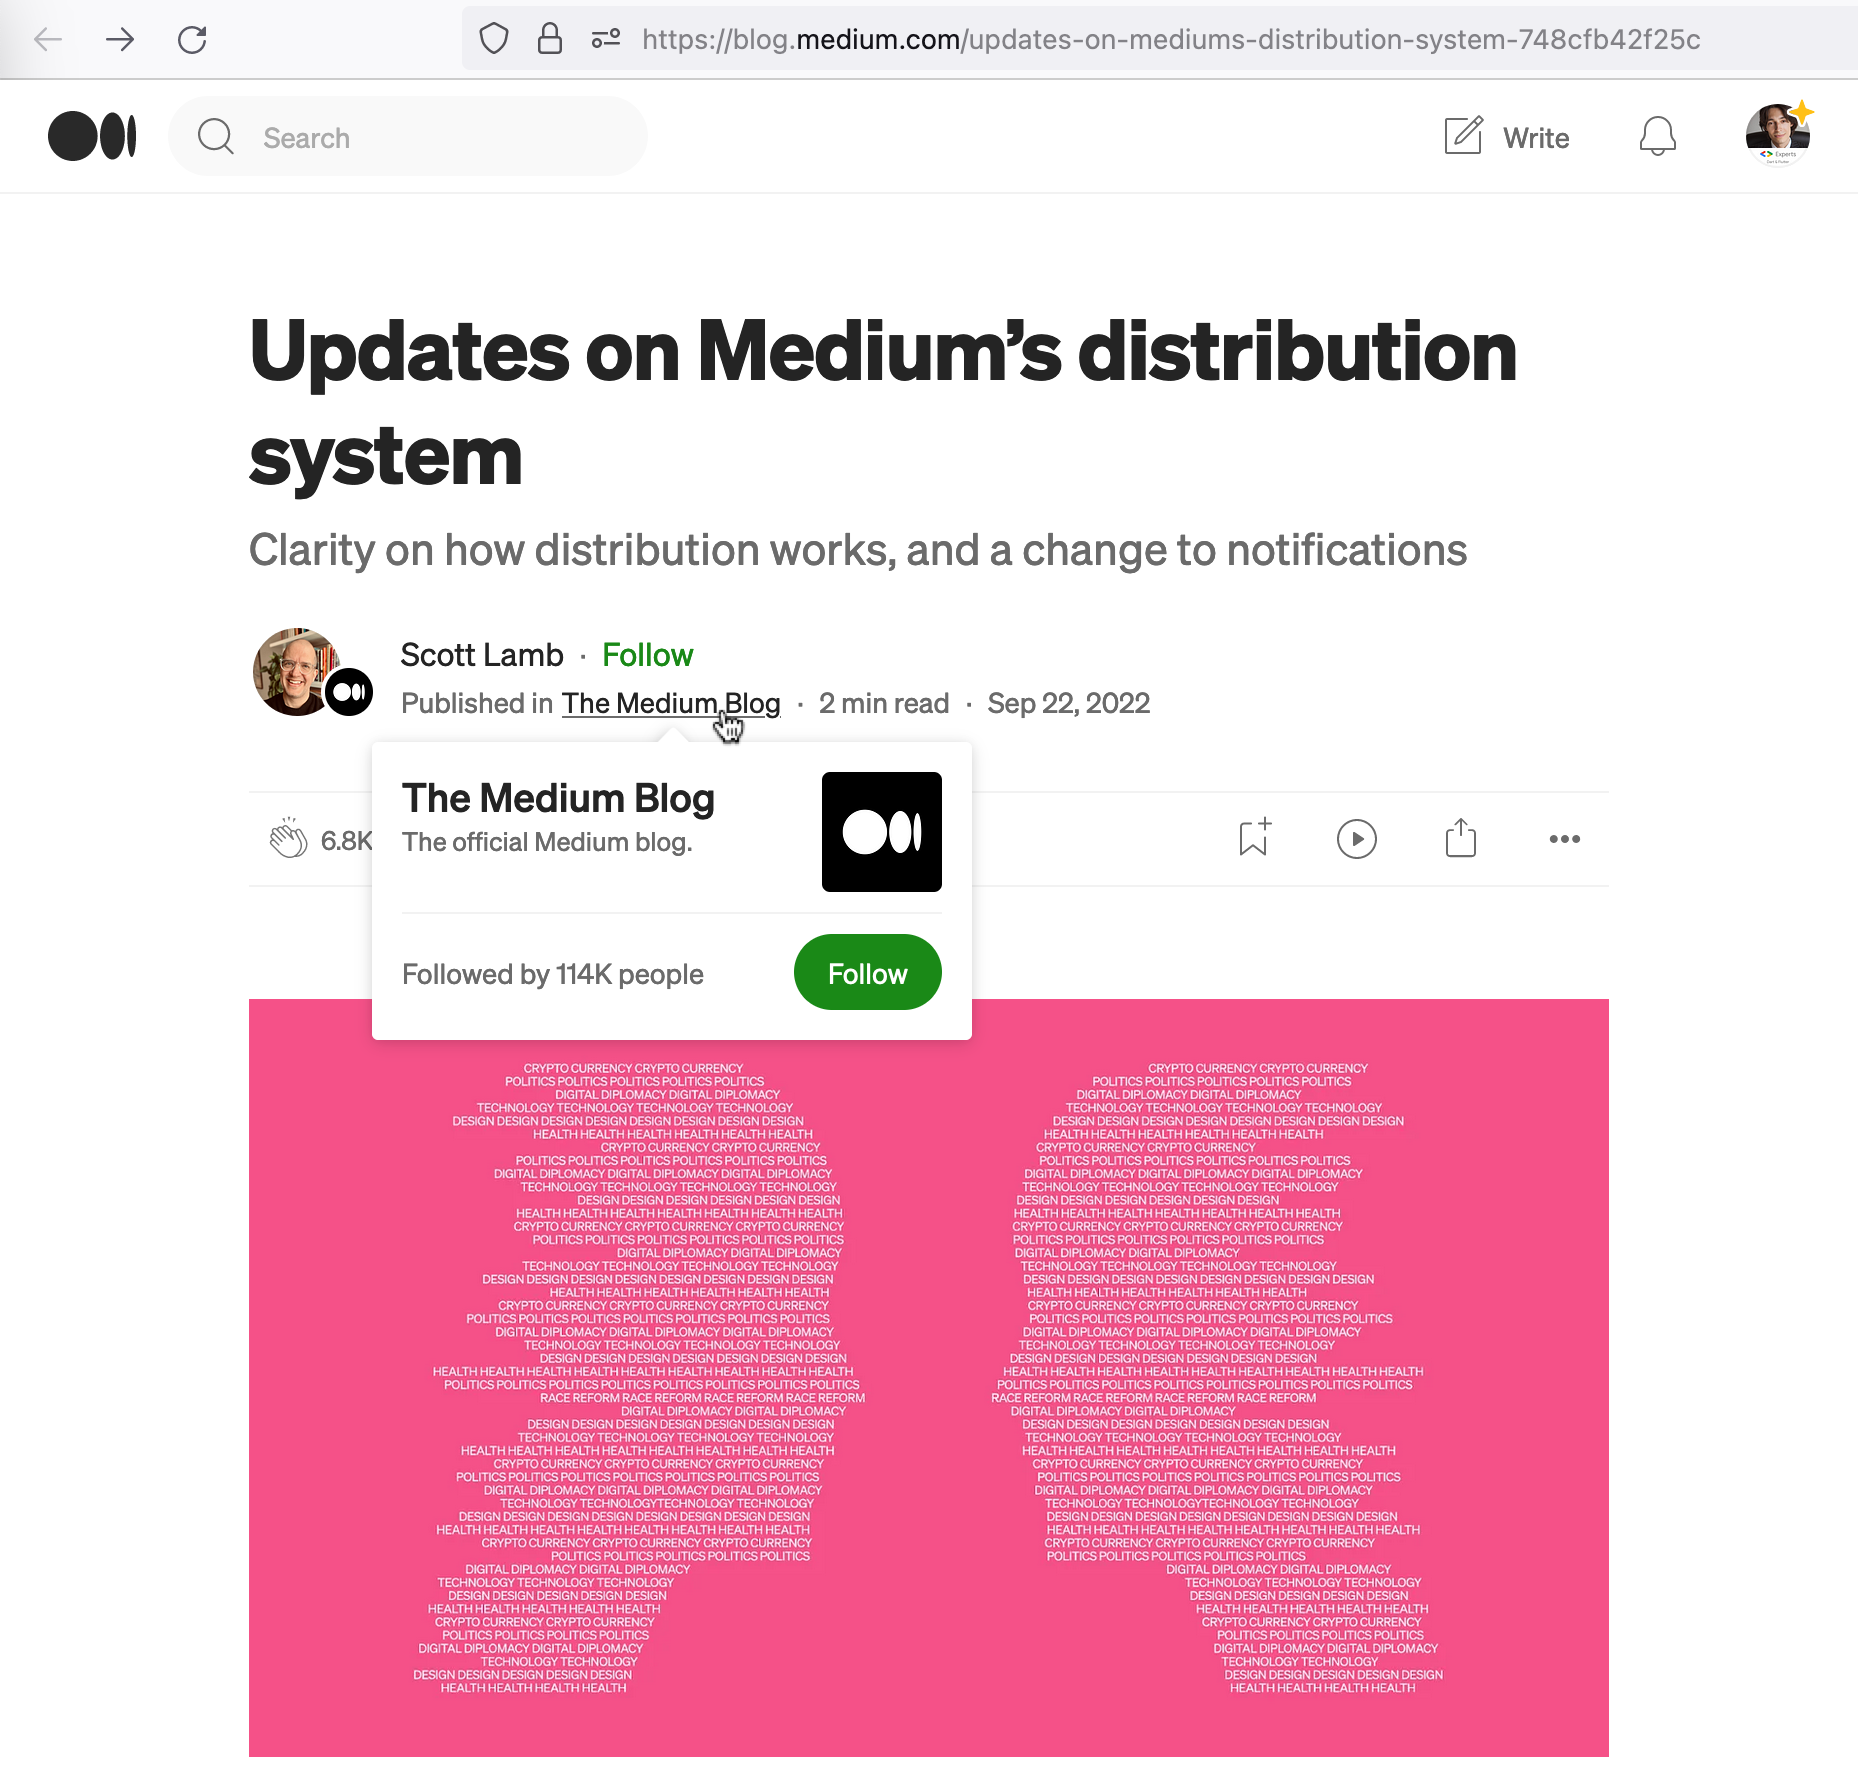
\includegraphics[width=38em]{no-more-p1}
\end{center}
\WillContinue
\pagebreak

\Continuing
\begin{center}
    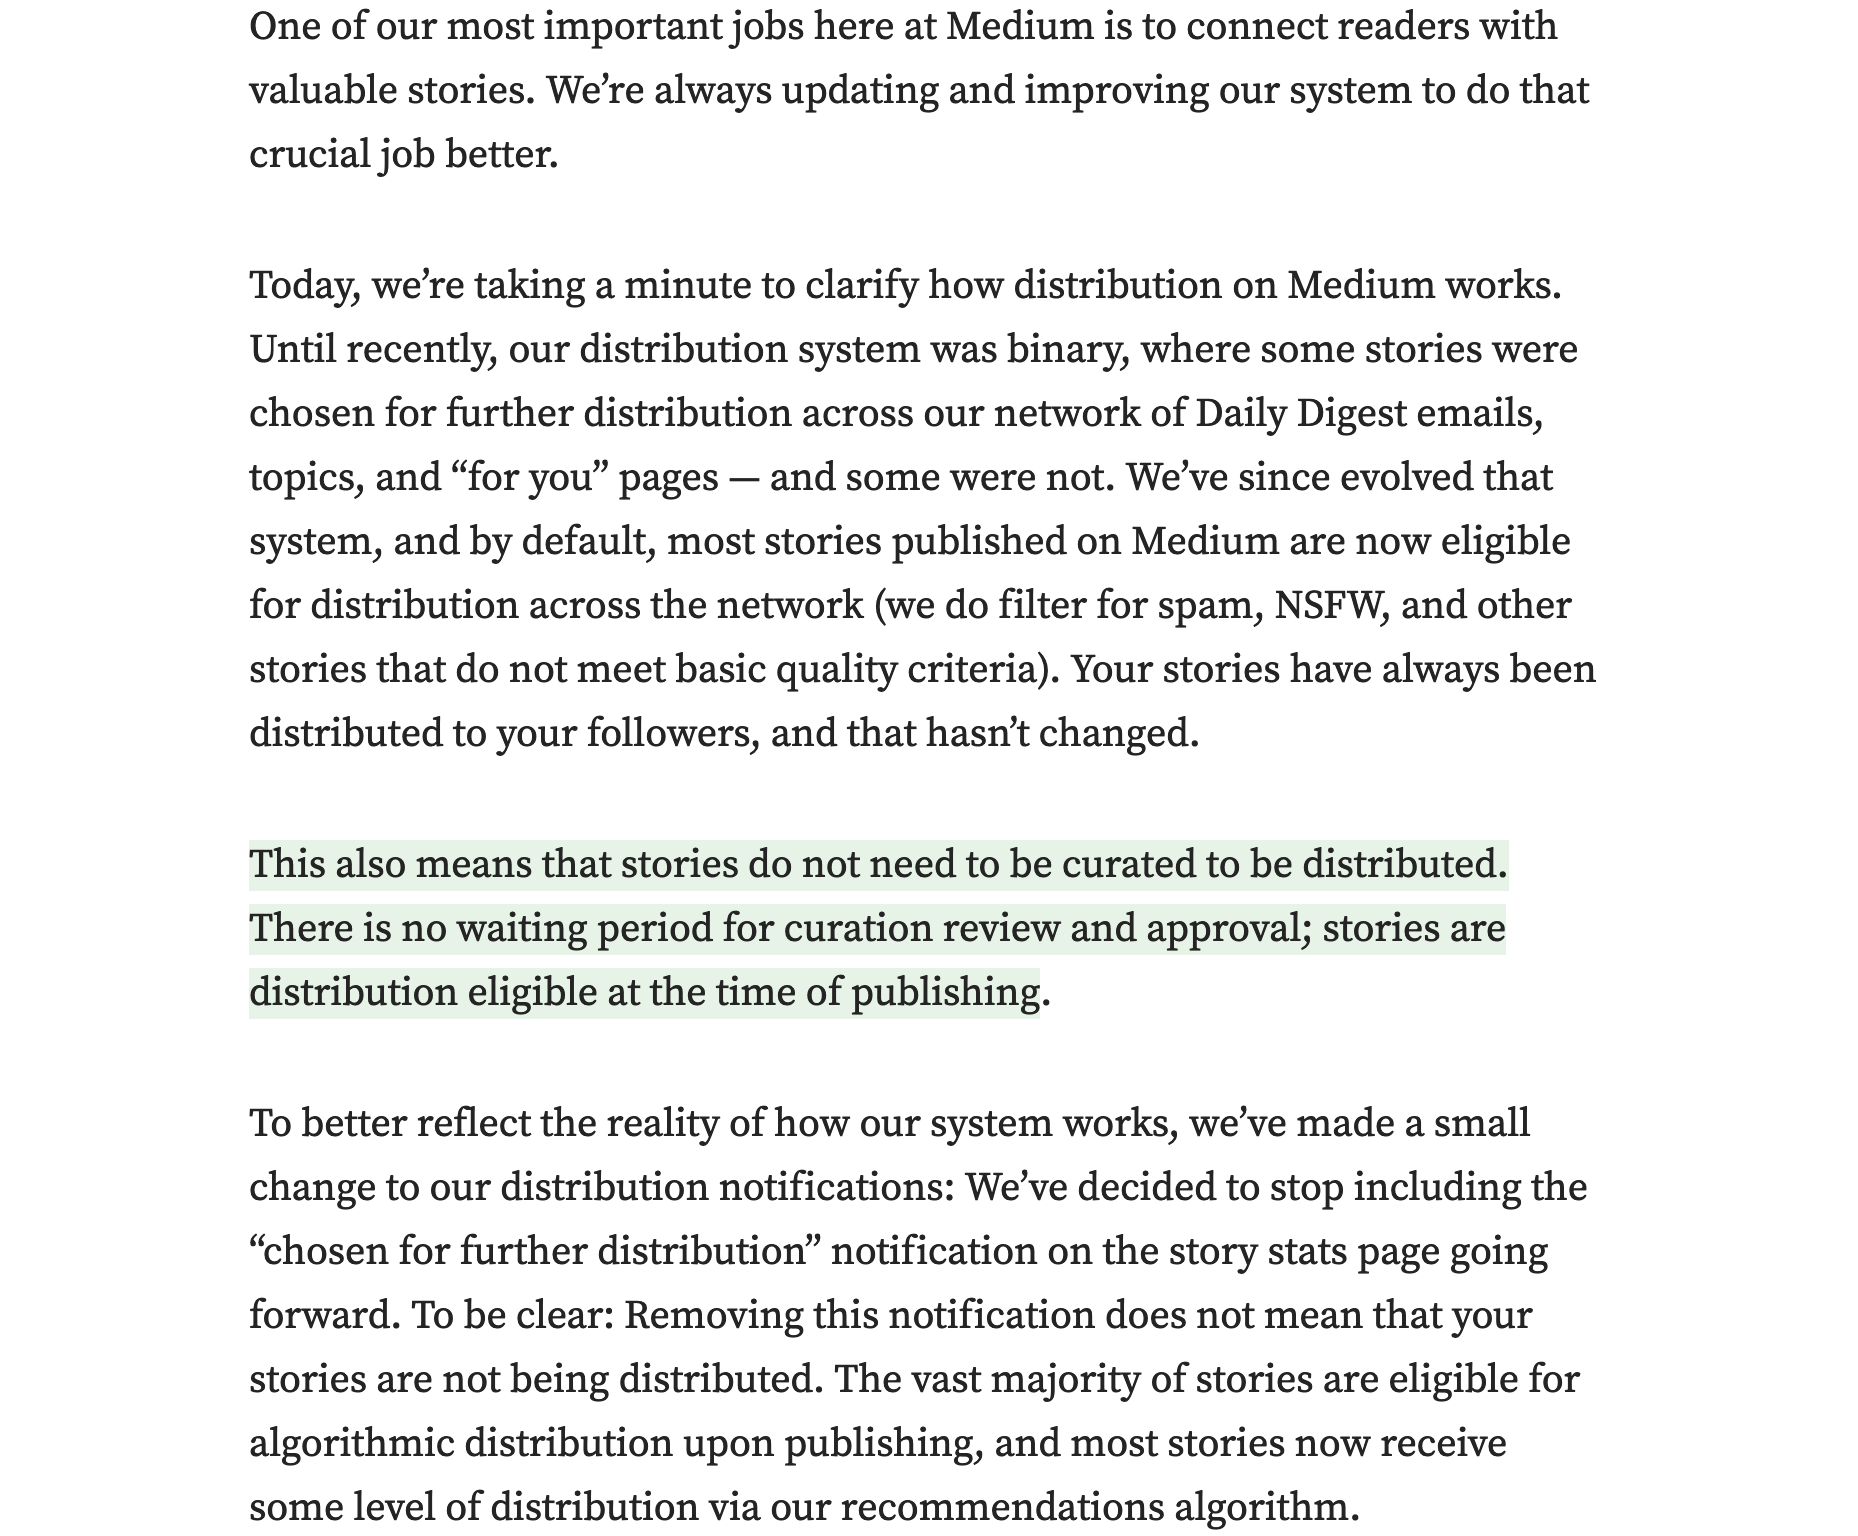
\includegraphics[width=\textwidth]{no-more-p2}
\end{center}

\pagebreak
